\chapter{Conclusione}
Tutte le varie architetture e tecniche analizzate in questo documento hanno i loro pro e contro. Nello stato attuale delle cose, è sicuramente vero che architetture come Flux e Redux, ossia a flusso unidirezionale, sono molto più gestibili e scalabili di architetture a flusso bidirezionale come quelle derivate da MVC.
Gran parte di ciò è vero però solo grazie all'incredibile innovazione apportata da React, o più in particolare dal Virtual DOM, al mondo delle applicazioni web ossia la capacità di modificare solamente gli elementi del DOM le cui proprietà sono effettivamente cambiate. Infatti sia Flux, che in particolare Redux, non sono in grado di fornire ai vari componenti informazioni su ciò che all'interno dello Store è stato cambiato bensì aggiornano blocchi di stato nel caso di Flux, e lo stato intero nel caso di Redux, causando una richiesta di modifica a molti più componenti di quelli che in realtà sono stati effettivamente cambiati.
Senza il Virtual DOM le prestazioni di queste architetture calerebbero in maniera non indifferente mettendo forse in ombra anche tutti i benefici strutturali da loro apportati, e magari l'architettura MVC in fin dei conti sarebbe ancora la scelta migliore.
Da questo punto di vista è possibile concludere che l'efficenza sia a livello di scalabilità, sia prestazionale di una architettura dipende dalle tecnologie presenti al tempo in cui essa viene adottata. Proprio per questo dire che Flux e Redux siano le architetture perfette per l'implementazione di applicazioni web complesse è sbagliato, è invece giusto dire che sono \textit{attualmente} perfette, con le tecnologie presenti fino a questo momento.

\begin{figure}[h]
\centering 
\vspace*{0.5cm} 
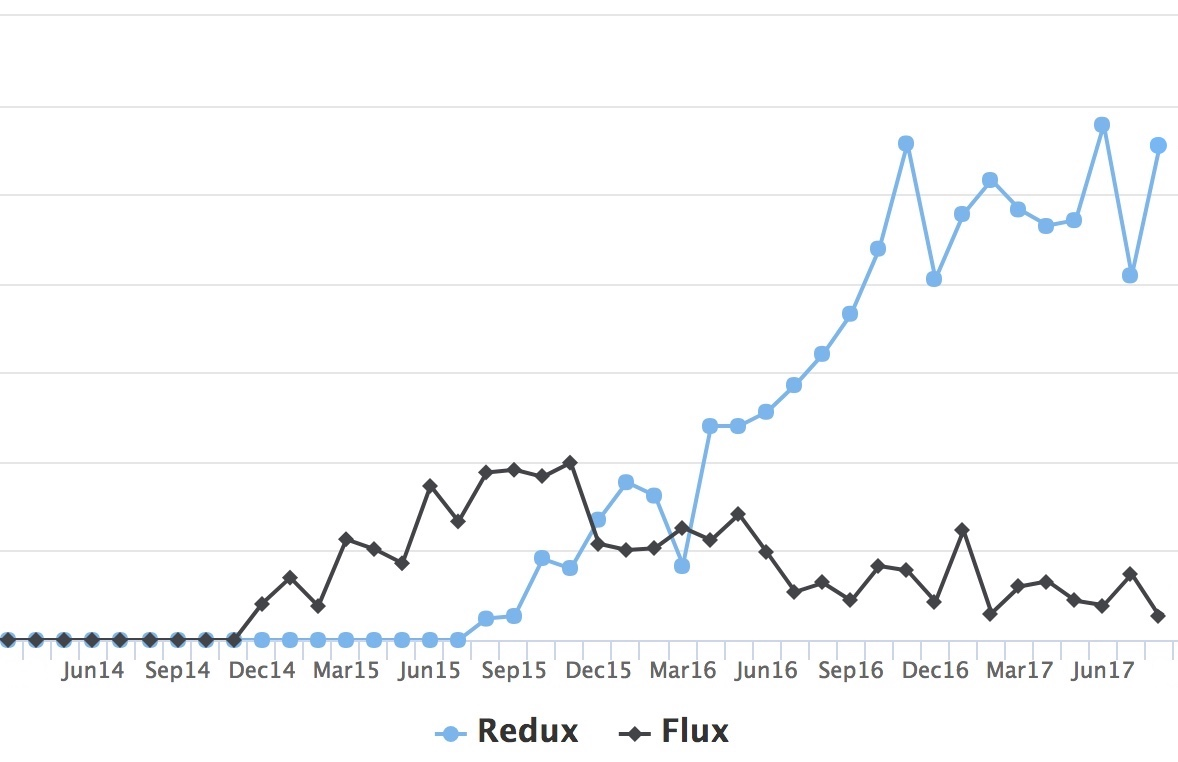
\includegraphics[width=11cm]{./images/fluxVsReduxPopularity}
\caption{Grafico della popolarità di Redux e Flux (generato da \href{https://www.hntrends.com/}{hntrends.com}).}
\label{fluxVsReduxPopularity}
\vspace*{0.5cm} 
\end{figure}

Riguardo alla “lotta” tra Flux e Redux (che come è possibile notare dalla Figura \ref{fluxVsReduxPopularity} attualmente sembra essere a senso unico) il giudizio spetta al programmatore. Analizzando solo l'architettura che permettono di organizzare, il vincitore sembrerebbe essere Redux, in quanto tutto ciò che fa è semplificare Flux utilizzando metodi alternativi (in questo caso pattern presi dalla programmazione funzionale) per la gestione dei dati. Tuttavia in questo documento molti argomenti di entrambe le architetture non sono stati toccati per il semplice fatto che avrebbero portato il discorso troppo fuori tema.
Uno di questi argomenti riguarda Redux, ed è la gestione di codice asincrono all'esecuzione di una Action. Come è stato più volte chiarito, il Reducer deve essere obbligatoriamente una funzione pura affinché l'architettura di Redux sia consistente, ciò pone ad esempio l'interrogativo del dove poter effettuare richieste HTTP ad una eventuale API. Questo problema viene brillantemente risolto da tecnologie come \textit{redux-thunk}\footnote{https://github.com/gaearon/redux-thunk}, \textit{redux-promise}\footnote{https://github.com/acdlite/redux-promise} o dal più recente \textit{redux-saga}\footnote{https://redux-saga.js.org/}. Queste librerie forniscono alternative differenti alla gestione di codice asincrono nell'architettura Redux. Tuttavia questo non basta ad una corretta gestione dell'applicazione. L'effettuare richieste asincrone causa un altro problema, questa volta relativo anche a Flux, ed è quello di cosa mostrare all'utente nel mentre della richiesta. L'analisi di queste librerie e la soluzione di questi problemi esulano dallo scopo di questo documento. La gestione del codice asincrono in Redux è un argomento vasto e complicato se analizzato in dettaglio e non apporta grossi vantaggi o svantaggi all'architettura in generale rispetto a quelli intrinsechi del paradigma. Il problema della gestione dell'interfaccia durante una richiesta asincrona invece è terreno comune ad entrambe le architetture come comuni sono le varie tecniche risolutive.

Al di là di questi problemi per prendere una decisione su quale architettura scegliere tra Flux e Redux sarebbe anche opportuno analizzare il loro ecosistema. Entrambe le architetture hanno attorno una community piuttosto attiva ed il numero di librerie e plugin implementati sia ufficialmente che dagli utenti è vasto.
In ultima battuta si può concludere che la scelta concreta tra queste due eventuali architetture, nonostante tenda un po' più verso Redux è anche una questione di preferenza del programmatore. Se un approccio funzionale è quello favorito e lavorare con dati immutabili non arreca alcun problema allora l'utilizzo di Redux è la scelta più ideale, altrimenti Flux potrebbe essere comunque una ottima alternativa.
